\begin{figure}[H]
    \centering
    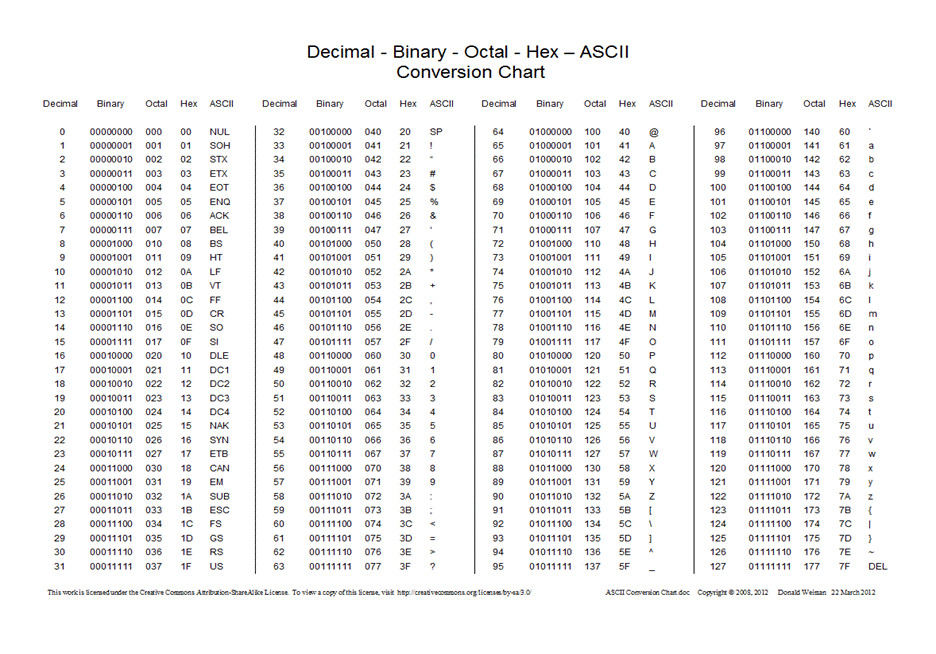
\includegraphics[width=0.8\textwidth]{code/pictures/Ascii.jpg}
    \caption{Ascii code}
    \label{Ascii}
\end{figure}
\begin{figure}[H]
    \centering
    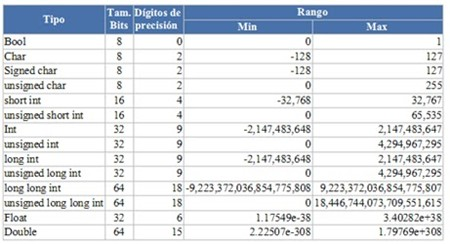
\includegraphics[width=0.6\textwidth]{code/pictures/DataTypes.jpg}
    \caption{Data types limits}
    \label{DataTypes}
\end{figure}
\begin{figure}[H]
    \centering
    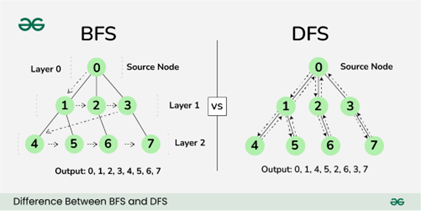
\includegraphics[width=0.6\textwidth]{code/pictures/dfs_bfs.png}
    \caption{DFS y BFS}
    \label{DFS_BFS}
\end{figure}

\begin{figure}[H]
    \centering
    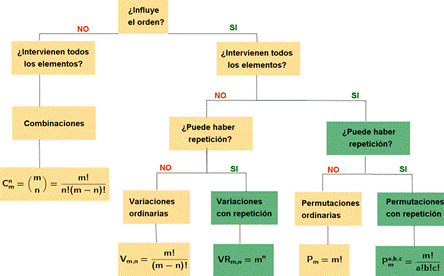
\includegraphics[width=0.6\textwidth]{code/pictures/Combinatorics.jpg}
    \caption{Combinatorics}
    \label{Combinatorics}
\end{figure}
\begin{figure}[H]
    \centering
    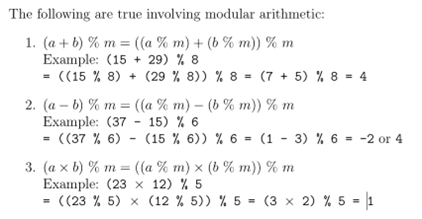
\includegraphics[width=0.6\textwidth]{code/pictures/Modulo_properties.png}
    \caption{Modulo properties}
    \label{Modulo_properties}
\end{figure}

\begin{figure}[H]
    \centering
    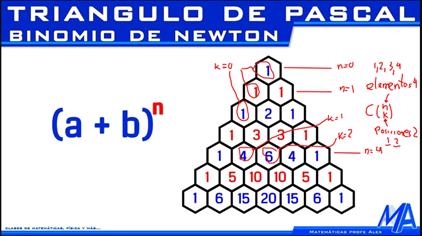
\includegraphics[width=0.6\textwidth]{code/pictures/Pascal_triangle.png}
    \caption{Pascal's triangle}
    \label{Pascal_triangle}
\end{figure}